%Master File:lectures.tex

\lesson{Optimisation}
\vspace{-1cm}
\begin{center}
\begin{center}
  \includegraphics[width=10cm]{grad-shade.png}\hfil%
  \includegraphics[width=10cm]{grad-contour.png}
\end{center}
\begin{displaymath}
z = \e{-(x+1)^2-(y-1)^2} + 0.6\,\e{-(x-1)^2-0.5(y+1)^2+0.1(x-3)(y-3)}
\end{displaymath}
\end{center}
\keywords{Gradient descent, quadratic minima, differing length scales}
%%%%%%%%%%%%%%%%%%%%%%% Next Slide %%%%%%%%%%%%%%%%%%%%%%%
\renewcommand{\Outline}{%
\begin{slide}
\section[1]{Outline}

\begin{minipage}{12cm}\raggedright
  \begin{enumerate}\squeeze
    \outlineitem{Motivation}{mot}
    \outlineitem{Gradient Descent}{descent}
    \outlineitem{Why Gradient Descent is Difficult}{difficult}
  \end{enumerate}
\end{minipage}\hfill
\begin{minipage}{10cm}
  \includegraphics[width=10cm]{grad-shade.png}
\end{minipage}
\end{slide}
\addtocounter{outlineitem}{1}
}

\setcounter{outlineitem}{1}

%%%%%%%%%%%%%%%%%%%%%%% Next Slide %%%%%%%%%%%%%%%%%%%%%%%
\Outline % Motivation
\toptarget{firstoutline}
%%%%%%%%%%%%%%%%%%%%%%% Next Slide %%%%%%%%%%%%%%%%%%%%%%%


\begin{slide}
\section{ML = Optimisation}

\begin{PauseHighLight}
\hypertarget{motivation}{}

\begin{itemize}
\item Many learning machines can be thought of as functions of the form
  \begin{displaymath}
    \hat{y} = f(\bm{x}|\bm{w})
  \end{displaymath}
  (or more generally $\hat{\bm{y}} = \bm{f}(\bm{x}|\bm{w})$)\pause
\item Given an input pattern (set of features) $\bm{x}$ the learning
  machine makes a prediction $\hat{y}$\pause
\item We try to choose the parameters $\bm{w}$ so that the predictions are
good\pause
\item In practice training a learning machine comes down to optimising
  some loss function\pause
\end{itemize}

\end{PauseHighLight}
\end{slide}

%%%%%%%%%%%%%%%%%%%%%%% Next Slide %%%%%%%%%%%%%%%%%%%%%%%

\begin{slide}
\section[-1.5]{MLP}

\begin{PauseHighLight}

\begin{itemize}
\item We can depict a neural network such as an MLP by a diagram
  \begin{center}
    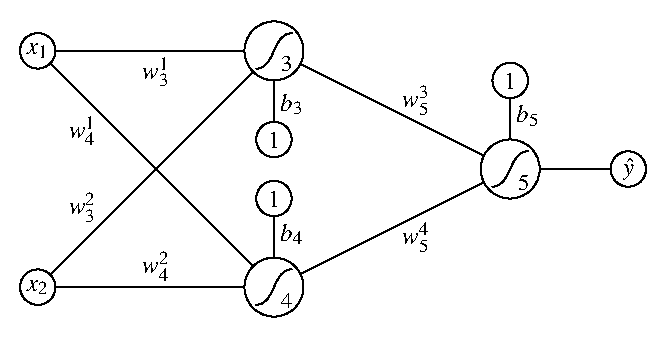
\includegraphics[height=7cm]{mlp-simple.eps}\pause
  \end{center}
\item Stands for the function ($\hat{y} = f(\bm{x}|\bm{w})$)
  \begin{displaymath}
    \hat{y} = g\!\left(w^3_5\, g(w^1_3\, x_1+w^2_3\,x_2+b_3) + w^4_5\, g(w^1_4\,
    x_1+w^2_4\,x_2+b_4) +b_5\right)
  \end{displaymath}
where, for example, $g(V) = \frac{1}{1+\e{-V}}$\pause
\end{itemize}

\end{PauseHighLight}
\end{slide}

%%%%%%%%%%%%%%%%%%%%%%% Next Slide %%%%%%%%%%%%%%%%%%%%%%%

\begin{slide}
\section{Training}

\begin{PauseHighLight}

\begin{itemize}
\item Given a (labelled) training dataset
  \begin{displaymath}
    \data = \left\{\strut (\bm{x}_k, y_k) \big| k=1,\ldots, m \right\} \pause
  \end{displaymath}
\item We define an error or loss function that we want to minimise
  \begin{displaymath}
    L(\bm{w|\data}) = \frac{1}{m} \sum_{k=1}^m \left( \strut
    f(\bm{x}_k|\bm{w}) - y_k \right)^2\pause
  \end{displaymath}
\item We then use the machine with the weights $\bm{w}^*$ which minimise
  $L(\bm{w}|\data)$\pause
\end{itemize}

\end{PauseHighLight}
\end{slide}

%%%%%%%%%%%%%%%%%%%%%%% Next Slide %%%%%%%%%%%%%%%%%%%%%%%

\begin{slide}
\section[-1]{Computing Gradients}

\begin{PauseHighLight}

\begin{itemize}
\item $L(\bm{w}|\data)$ is a complex function of the weights $\bm{w}$
  \begin{center}
    \includegraphics[height=7cm]{rough_landscape}\pause
  \end{center}
\item To minimise we $L(\bm{w}|\data)$ we compute the gradient $\grad
  L(\bm{w}|\data)$\pause 
\item In MLP an efficient algorithm for computing the gradient is known as
  back-prop\pause
\end{itemize}

\end{PauseHighLight}
\end{slide}


%%%%%%%%%%%%%%%%%%%%%%% Next Slide %%%%%%%%%%%%%%%%%%%%%%%
\Outline % Gradient descent
%%%%%%%%%%%%%%%%%%%%%%% Next Slide %%%%%%%%%%%%%%%%%%%%%%%

\begin{slide}
\section[-2]{Gradient Optimisation}

\begin{PauseHighLight}
\hypertarget{descent}{}

\begin{itemize}\squeeze
\item A maximum or minimum occurs when $\grad L(\bm{w}|\data)=\bm{0}$\pause
\item E.g.
\begin{displaymath}
z = \e{-(x+1)^2-(y-1)^2} + 0.6\,\e{-(x-1)^2-0.5(y+1)^2+0.1(x-3)(y-3)}
\end{displaymath}
  \begin{center}
  \includegraphics[width=10cm]{grad-shade.png}\hfil%
  \includegraphics[width=14cm]{grad-contour.png}   \pause 
  \end{center}
\end{itemize}
\end{PauseHighLight}
\end{slide}

%%%%%%%%%%%%%%%%%%%%%%% Next Slide %%%%%%%%%%%%%%%%%%%%%%%

\begin{slide}
\section{Gradient Descent}

\begin{PauseHighLight}

\begin{itemize}
\item For a simple function $L(\bm{w}|\data)$ we can solve $\grad
  L(\bm{w}|\data)=\bm{0}$ explicitly\pause.  E.g. the linear perceptron\pause
\item For a non-linear functions we usually can't solve this set of
  simultaneous equations\pause
\item We can find a maximum or minimum \textbf{iteratively}\pause
\item If we know the gradient then we can follow the gradient\pause
  \begin{itemize}
  \item Maximisation: $\bm{w} \rightarrow \bm{w}'=\bm{w}+r \grad
    L(\bm{w}|\data)$ \pause
  \item Minimisation: $\bm{w} \rightarrow \bm{w}'=\bm{w}-r \grad
    L(\bm{w}|\data)$ \pause
  \end{itemize}
\end{itemize}


\end{PauseHighLight}
\end{slide}

%%%%%%%%%%%%%%%%%%%%%%% Next Slide %%%%%%%%%%%%%%%%%%%%%%%

\begin{slide}
\section[-2]{Hill-Climbing}

\pb
\begin{center}
  \thicklines
  \setlength{\unitlength}{1.1mm}
  \begin{picture}(200,150)
    \put(0,0){\includegraphics[width=200\unitlength]{grad-contour.png}}
    \put(87,67){\textcolor{red}{\circle*{2}}}\pause
    \put(87,67){\textcolor{black}{\line(1,1){4}}}
    \put(90,70){\textcolor{red}{\circle*{2}}}\pause
    \put(90,70){\textcolor{black}{\line(1,2){4}}}
    \put(94,78){\textcolor{red}{\circle*{2}}}\pause
    \put(94,78){\textcolor{black}{\line(1,3){2}}}
    \put(96,84){\textcolor{red}{\circle*{2}}}\pause
    \put(96,84){\textcolor{black}{\line(-1,1){6}}}
    \put(90,90){\textcolor{red}{\circle*{2}}}\pause
    \put(90,90){\textcolor{black}{\line(-3,2){5}}}
    \put(85,93){\textcolor{red}{\circle*{2}}}\pause
  \end{picture}
\end{center}

\end{slide}

%%%%%%%%%%%%%%%%%%%%%%% Next Slide %%%%%%%%%%%%%%%%%%%%%%%

\begin{slide}
\section[-2]{What Goes Right}

\begin{PauseHighLight}

\begin{itemize}\squeeze
\item Almost all minima are quadratic\pause\ (Morse's theorem)\pause
  \begin{center}
    \includegraphics[width=9cm]{morse.eps}
  \end{center}
\item Taylor expanding around a minimum $x^*$
  \begin{eqnarray*}
    f(x) &=& f(x^*) + (x-x^*)\, f'(x^*) + \frac{1}{2}
    \left(x-x^*\right)^2\, f''(x^*) + \cdots\pause \\
    &=& f(x^*) + \frac{1}{2} \left(x-x^*\right)^2\,f''(x^*)
     + \frac{1}{3!} \left(x-x^*\right)^3 \,f'''(x^*) + \cdots \pause
  \end{eqnarray*}
\item If $x-x^*$ is sufficiently small the higher order terms are
  negligible\pause 
\end{itemize}
\end{PauseHighLight}
\end{slide}

%%%%%%%%%%%%%%%%%%%%%%% Next Slide %%%%%%%%%%%%%%%%%%%%%%%

\begin{slide}
\section{Newton's Method}

\begin{PauseHighLight}

\begin{itemize}
\item If we were in a quadratic minimum
  \vspace{-2cm}
  \begin{displaymath}
    f(x) = a + \frac{b}{2} \left(x-x^*\right)^2 \hspace{3cm}
    \raisebox{-1cm}{\includegraphics[width=7cm]{quadratic}}
 \pause
  \end{displaymath}
\item then
  \begin{displaymath}
    f'(x) = b\,\left(x-x^*\right), \hspace{2em}
    f''(x) = b\pause
  \end{displaymath}
\item so
  \begin{displaymath}
    x-x^* = \frac{f'(x)}{b} = \frac{f'(x)}{f''(x)}\pause
  \end{displaymath}
\item or
  \begin{displaymath}
    x^* = x - \frac{f'(x)}{f''(x)}\pause
  \end{displaymath}
\end{itemize}

\end{PauseHighLight}
\end{slide}

%%%%%%%%%%%%%%%%%%%%%%% Next Slide %%%%%%%%%%%%%%%%%%%%%%%

\begin{slide}
\section{Newton's Method}

\begin{PauseHighLight}

\begin{itemize}
\item This is Newton's methods\pause
\item For non-quadratic functions Newtons method converges
  \textbf{quadratically} provided we are sufficiently close to a minimum\pause
\item If we are at a distance $x-x^*=\epsilon$ from the minima then after
  one cycle we will be a distance $\epsilon^2$\pause\ after two cycles we
  will be at a distance $\epsilon^4$, etc.\pause
\item If we are too far from a minimum we might go anywhere!\pause
\item We should follow the gradient until we are near the minimum\pause
\end{itemize}

\end{PauseHighLight}
\end{slide}

%%%%%%%%%%%%%%%%%%%%%%% Next Slide %%%%%%%%%%%%%%%%%%%%%%%

\begin{slide}
\section[-1.5]{Taylor's Expansion in High Dimensions}

\begin{PauseHighLight}

\begin{itemize}\squeeze
\item We can generalise these results to many dimensions\pause
\item The Taylor expansion of a function $f(\bm{x})$ about $\bm{x}_0$
  \begin{displaymath}
        f(\bm{x}) = f(\bm{x}_0) + \left(\bm{x}-\bm{x}_0\right)^\tr\,
    \grad f(\bm{x}_0) + \frac{1}{2} \left(\bm{x}-\bm{x}_0\right)^\tr\,
    \mat{H} \left(\bm{x}-\bm{x}_0\right) + \cdots\pause
  \end{displaymath}
  where $\mat{H}$ is the \textbf{Hessian} matrix with elements
  \begin{displaymath}
    H_{ij} = \frac{\partial^2 f(\bm{x}_0)}{\partial x_i \,\partial x_j}
    \pause 
  \end{displaymath}
\item Newton's method in high dimension is
  \begin{displaymath}
    \bm{x}^* = \bm{x} - \mat{H}^{-1} \, \grad \,f(\bm{x})\pause
  \end{displaymath}
\end{itemize}

\end{PauseHighLight}
\end{slide}

%%%%%%%%%%%%%%%%%%%%%%% Next Slide %%%%%%%%%%%%%%%%%%%%%%%

\begin{slide}
\section[-1]{Using the Second Derivative}

\begin{PauseHighLight}

\begin{itemize}\squeeze
\item If we are optimising $N$ parameters the Hessian is an $N\times N$
  matrix\pause
\item It is time-consuming to compute\pause\ (and prone to errors when
  coding)\pause---for deep learning it is impossible even to store the
  Hessian\pauseb
\item Away from minima they can be misleading
  \begin{center}
    \includegraphics[width=20cm]{hess-missleading}\pause
  \end{center}
\end{itemize}

\end{PauseHighLight}
\end{slide}


%%%%%%%%%%%%%%%%%%%%%%% Next Slide %%%%%%%%%%%%%%%%%%%%%%%
\Outline % What goes wrong
%%%%%%%%%%%%%%%%%%%%%%% Next Slide %%%%%%%%%%%%%%%%%%%%%%%

\begin{slide}
\section{Step Size}

\begin{PauseHighLight}

\begin{itemize}\squeeze
\item Gradient descent
  \begin{displaymath}
    \bm{x}' = \bm{x} - r \, \grad \,f(\bm{x})\pause
  \end{displaymath}
\item Need to choose the learning rate of step size, $r$\pause
\item Too small steps takes lots of time\pause
\item Too large steps takes you away from a minimum\pause
\end{itemize}

\end{PauseHighLight}
\end{slide}

%%%%%%%%%%%%%%%%%%%%%%% Next Slide %%%%%%%%%%%%%%%%%%%%%%%


\begin{slide}
\section[1]{Step Size}

\pb
\begin{center}
  \includegraphics[width=\linewidth]{minquad-bg}\pause
  \multido{\ia=0+1}{28}{%
    \llap{\includegraphics[width=\linewidth]{minquad-\ia}}\pause}
\end{center}
\end{slide}

%%%%%%%%%%%%%%%%%%%%%%% Next Slide %%%%%%%%%%%%%%%%%%%%%%%

\begin{slide}
\section{Higher Dimensions}

\pb
\begin{itemize}
\item In higher dimensions the problem is that there are some directions
  you need to move a long way\pauseh
\end{itemize}
\begin{center}
  \includegraphics[width=\linewidth]{min2d-bg}\pause
  \multido{\ia=0+1}{10}{%
    \llap{\includegraphics[width=\linewidth]{min2d20-\ia}}\pause}
\end{center}
\end{slide}

%%%%%%%%%%%%%%%%%%%%%%% Next Slide %%%%%%%%%%%%%%%%%%%%%%%

\begin{slide}
\section{Getting There Quicker}

\pb
\begin{itemize}
\item Increasing the step size speeds up convergence, but the direction
  of steepest descent doesn't point to the minimum\pauseh
\end{itemize}
\begin{center}
  \includegraphics[width=\linewidth]{min2d-bg}\pause
  \multido{\ia=0+1}{10}{%
    \llap{\includegraphics[width=\linewidth]{min2d30-\ia}}\pause}
\end{center}
\end{slide}

%%%%%%%%%%%%%%%%%%%%%%% Next Slide %%%%%%%%%%%%%%%%%%%%%%%

\begin{slide}
\section{More Haste Less Speed}

\pb
\begin{itemize}
\item Increasing the step size, just a little further, increases the
  rate of converge in one direction, but \ldots\pauseh
\end{itemize}
\begin{center}
  \includegraphics[width=\linewidth]{min2d-bg}\pause
  \multido{\ia=0+1}{10}{%
    \llap{\includegraphics[width=\linewidth]{min2d35-\ia}}\pause}
\end{center}

\end{slide}



%%%%%%%%%%%%%%%%%%%%%%% Next Slide %%%%%%%%%%%%%%%%%%%%%%%

\begin{slide}
\section{Line Minimisation}

\begin{itemize}
\item We can systematically seek the minimum along a line of the
  gradient\pauseh
\end{itemize}
\begin{center}
  \includegraphics[width=\linewidth]{min2d-bg}\pause
  \multido{\ia=0+1}{10}{%
    \llap{\includegraphics[width=\linewidth]{linemin-\ia}}\pause}
\end{center}
\end{slide}

%%%%%%%%%%%%%%%%%%%%%%% Next Slide %%%%%%%%%%%%%%%%%%%%%%%

\begin{slide}
\section[-2]{Zig-Zag}

\begin{PauseHighLight}
  \begin{itemize}
  \item Note that in high dimensions gradient descent tends to zigzag
    \begin{center}
      \includegraphics[width=0.5\linewidth]{min2d-bg}\pause
      \multido{\ia=0+1}{10}{%
        \llap{\includegraphics[width=0.5\linewidth]{linemin-\ia}}}\pause
    \end{center}
  \item If we computed the Hessian and used Newton's method we would
    jump straight to the minimum if we were in a quadratic potential\pause
  \item However computing the Hessian is time consuming and misleading
    if we are not in a quadratic potential (i.e. far from the optimum)\pause
  \end{itemize}
\end{PauseHighLight}

\end{slide}


%%%%%%%%%%%%%%%%%%%%%%% Next Slide %%%%%%%%%%%%%%%%%%%%%%%

\begin{slide}
\section[-1]{Best Optimisation Algorithms}

\begin{PauseHighLight}

\begin{itemize}
\item The best optimisation algorithms compute an approximation of the
  Hessian\pause
\item E.g. Conjugate gradient\pause
  \begin{itemize}\squeeze
  \item Performs Line Minimisation\pause
  \item Uses gradient, but does not go along it\pause
  \item Reaches quadratic minimum in $N$ steps\pause
  \end{itemize}
\item E.g. Levenberg-Marquardt\pause
  \begin{itemize}\squeeze
  \item Used on least squares problem only\pause
  \item Uses linear approximation of function to approximate Hessian\pause
  \item Adapts from hill-climbing to Newton method\pause
  \item Avoids line-minimisation\pause
  \end{itemize}
\end{itemize}

\end{PauseHighLight}
\end{slide}

%%%%%%%%%%%%%%%%%%%%%%% Next Slide %%%%%%%%%%%%%%%%%%%%%%%

\begin{slide}
\section[-2]{Levenberg-Marquardt}

\begin{PauseHighLight}
  \begin{itemize}
  \item Want to minimise $\|\bm{\epsilon}(\bm{w})\|^2$ where
    $\epsilon_i(\bm{w}) =  f(\bm{x}_i|\bm{w}) - y_i$\pause
  \item Use linear approximation
    \begin{align*}
      \epsilon_i(\bm{w}) \approx \epsilon_i(\bm{w}^{(k)}) +
      (\bm{w}-\bm{w}^{(k)}) \grad \epsilon_i(\bm{w}^{(k)})
    \end{align*}
    with $\grad \epsilon_i(\bm{w}^{(k)}) = \grad f(\bm{x}_i|\bm{w}^{(k)})$\pause
  \item Solve quadratic minimisation of approximate error
    $\mathop{\mathrm{argmin}}_{\bm{w}} 
    L_{approx}(\bm{w})$ with $\mat{J}=\grad \bm{\epsilon}(\bm{w}^{(k)})$
    \begin{align*}
      L_{approx}(\bm{w}) &= 
      \| \bm{\epsilon}(\bm{w}^{(k)}) +
      \mat{J} (\bm{w}-\bm{w}^{(k)}) \|^2 \\
      &=
      \bm{\epsilon}(\bm{w}^{(k)})^\tr\bm{\epsilon}(\bm{w}^{(k)})
      + 2 (\bm{w}-\bm{w}^{(k)})^\tr \mat{J}^\tr
      \bm{\epsilon}(\bm{w}^{(k)}) \\
      &\hspace{2em}
      + (\bm{w}-\bm{w}^{(k)})^\tr \mat{J}^\tr \mat{J} (\bm{w}-\bm{w}^{(k)})
      \pause
    \end{align*}
  \end{itemize}
\end{PauseHighLight}

\end{slide}

%%%%%%%%%%%%%%%%%%%%%%% Next Slide %%%%%%%%%%%%%%%%%%%%%%%

\begin{slide}
\section[-1]{Trust Region}

\begin{PauseHighLight}
  \begin{itemize}
  \item Solution given by $\grad_{\bm{w}} L_{approx}(\bm{w}) = 0$ gives
    \begin{align*}
      \bm{w}^{(k+1)} = \bm{w}^{(k)} -
      \left(\mat{J}^\tr\mat{J}\right)^{-1} \mat{J}^\tr
      \bm{\epsilon}(\bm{w}^{(k)})\pause
    \end{align*}
  \item Can lead us in the wrong direction\pause
  \item Instead use $\bm{w}^{(k+1)}= \mathop{\mathrm{argmin}}_{\bm{w}} L_{approx}(\bm{w}) + \nu
    \|\bm{w}-\bm{w}^{(k)}\|^2$
    \begin{align*}
      \bm{w}^{(k+1)} = \bm{w}^{(k)} -
      \left(\mat{J}^\tr\mat{J} + \nu \mat{I}\right)^{-1} \mat{J}^\tr
      \bm{\epsilon}(\bm{w})\pause
    \end{align*}
  \item $\nu$ limits the step size\pause
  \item If predicted reduction in error is accurate reduce $\nu$, if
    predicted reduction in error is very poor increase $\nu$\pause
  \end{itemize}
\end{PauseHighLight}

\end{slide}

%%%%%%%%%%%%%%%%%%%%%%% Next Slide %%%%%%%%%%%%%%%%%%%%%%%

\begin{slide}
\section[-2]{$\epsilon_1 = 10\,(x_2-x_1^2)$ and $\epsilon_2=1-x_1$}
\pb\pause
\begin{center}
  \includegraphics[width=0.9\linewidth]{lm1}\mypl{1}
  \multido{\i=1+1}{6}{%
    \llap{\includegraphics[width=0.9\linewidth]{lm\i}\mypl{\i}}}
\end{center}

\end{slide}


%%%%%%%%%%%%%%%%%%%%%%% Next Slide %%%%%%%%%%%%%%%%%%%%%%%

\begin{slide}
\section[-1.5]{Landscape Problems}

\begin{PauseHighLight}

\begin{itemize}\squeeze
\item For sigmoid response function such as the logistic or tanh
  function there are very flat regions away from the bias\pause
\item Very little gradient information (can use momentum)\pause
\item Many local minima\pause---not guaranteed to find global minimum\pause
\item Weight space is symmetric because of permutation symmetry
  \begin{center}
    \includegraphics[width=10cm]{mlp.eps}\pause
  \end{center}
\end{itemize}

\end{PauseHighLight}
\end{slide}

%%%%%%%%%%%%%%%%%%%%%%% Next Slide %%%%%%%%%%%%%%%%%%%%%%%

\begin{slide}
\section[-2]{Saddle-Points}

\pb
\begin{itemize}
\item Many saddle-points due to permutation symmetry of hidden nodes\pauseh
  \begin{center}
    \includegraphics[width=17cm]{saddlept2}\pauseh
  \end{center}
\end{itemize}

\end{slide}

%%%%%%%%%%%%%%%%%%%%%%% Next Slide %%%%%%%%%%%%%%%%%%%%%%%

\begin{slide}
\section{Modern Machine Learning}

\begin{PauseHighLight}
  \begin{itemize}
  \item Modern deep learning machines usually have so many parameters
    that it would be impractical to even estimate the Hessian\pause
  \item We now commonly use ReLU's rather than sigmoids so the cost
    landscape is non-analytic\pause
  \item Making assumptions about the minima being quadratic is no
    longer true\pause
  \item In deep learning it is usually important to ensure that loss
    is differentiable almost everywhere\pause{} otherwise we can't use
    gradient descent\pauseb
  \end{itemize}
\end{PauseHighLight}

\end{slide}

%%%%%%%%%%%%%%%%%%%%%%% Next Slide %%%%%%%%%%%%%%%%%%%%%%%

\begin{slide}
\section{Summary}

\begin{PauseHighLight}
\label{last}

\begin{itemize}
\item Minimising the error gives a general purpose learning algorithm
  \begin{itemize}
  \item E.g.\ Logistic Perceptron, Multi-Layer Perceptron, CNNs, \ldots\pause
  \end{itemize}
\item The minimisation is in a high dimensional space\pause
\item Minimisation can be very time consuming\pause
\item Nasty things can happen, but there are many standard algorithms which
  work well\pause
\item In complex models there may be many minima\pause---you are not
  guaranteed to find the best one\pause
\end{itemize}


\end{PauseHighLight}
\end{slide}



%%% Local Variables:
%%% TeX-master: "lectures"
%%% End:
